\specialsection{Заключение}

В рамках выпускной квалификационной работы был разработан комплекс информационных систем
для проведения соревнований и тренировок по спортивному программированию в формате дуэлей.
Разработанная система поддерживает проведение рейтинговых и дружеских дуэлей, управление группами пользователей,
организацию турниров, автоматическое тестирование решений, а также анализ поведения участников во время решения задач.

Пользовательский Web-интерфейс позволяет пользователям входить в систему,
участвовать в дуэлях, использовать функционал групп и турниров.
Пример интерфейса участия в дуэли представлен на рисунке \ref{duel-interface}.
На экране дуэли отображаются редактор кода, условие задачи, доступные тесты и элементы управления запуском решения.

\begin{figure}[ht]
\begin{center}
\scalebox{0.3}{
   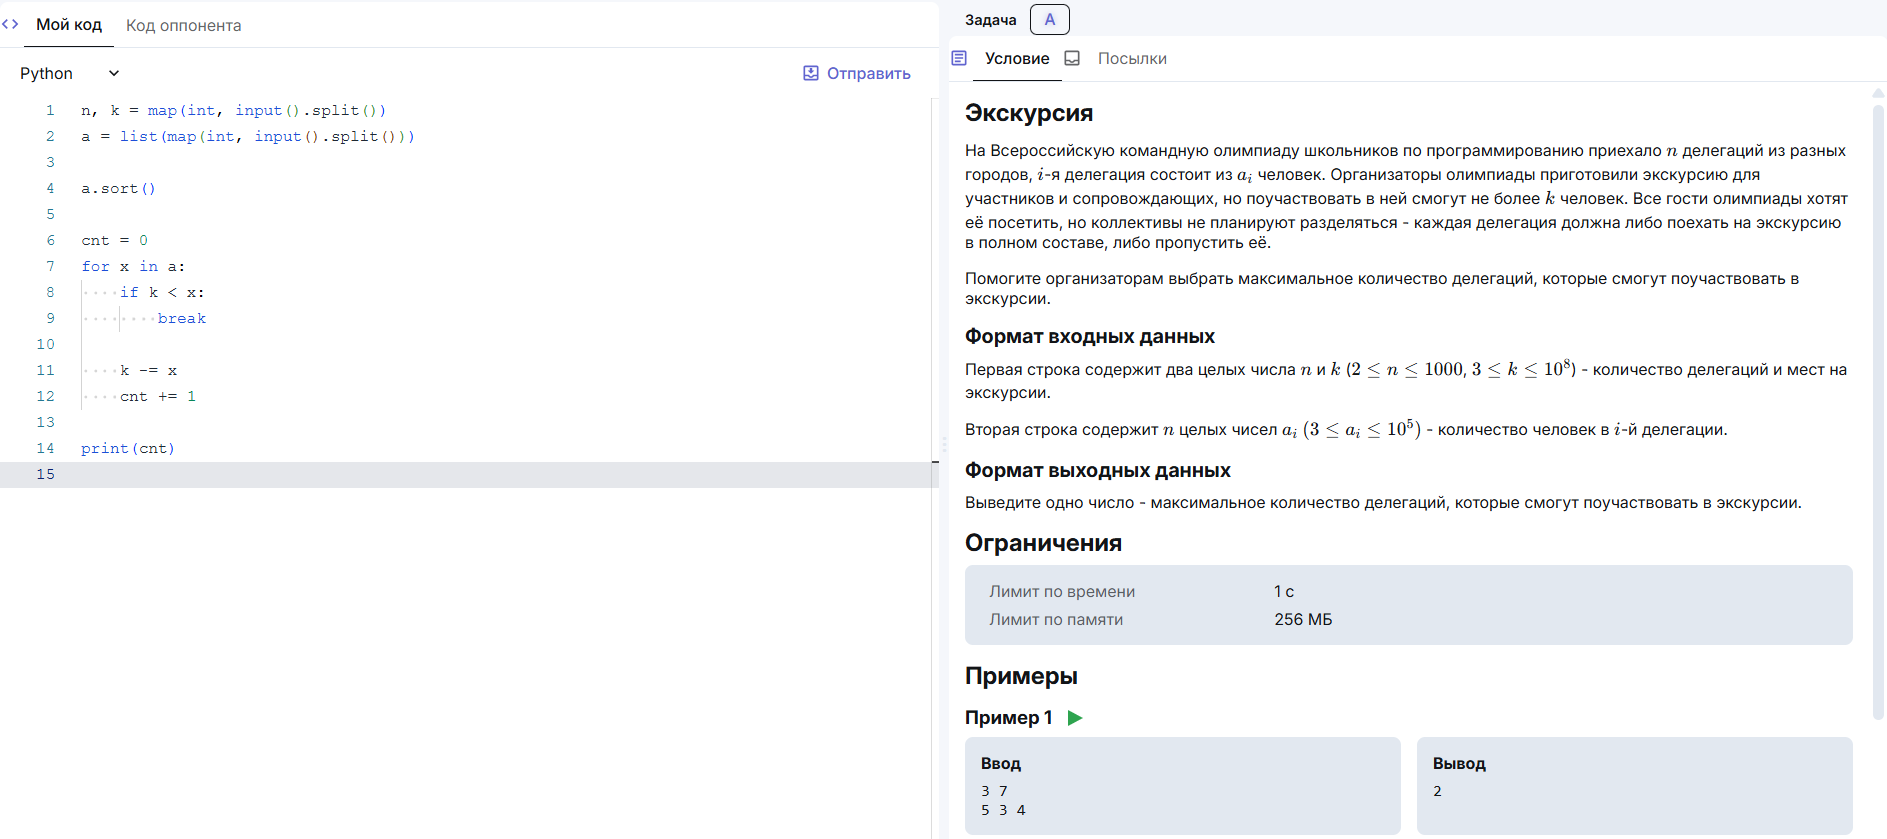
\includegraphics{images/duel-interface.png}
}
\caption{
\label{duel-interface}
     Интерфейс участия в дуэли.}
\end{center}
\end{figure}

Также в качестве примера интерфейса на рисунке \ref{tournament-interface} показан экран с результатами турнира, проведенного в СПбГУ.
На интерфейсе отображается турнирная таблица, а также результаты дуэлей между участниками турнира.

\begin{figure}[ht]
\begin{center}
\scalebox{0.6}{
   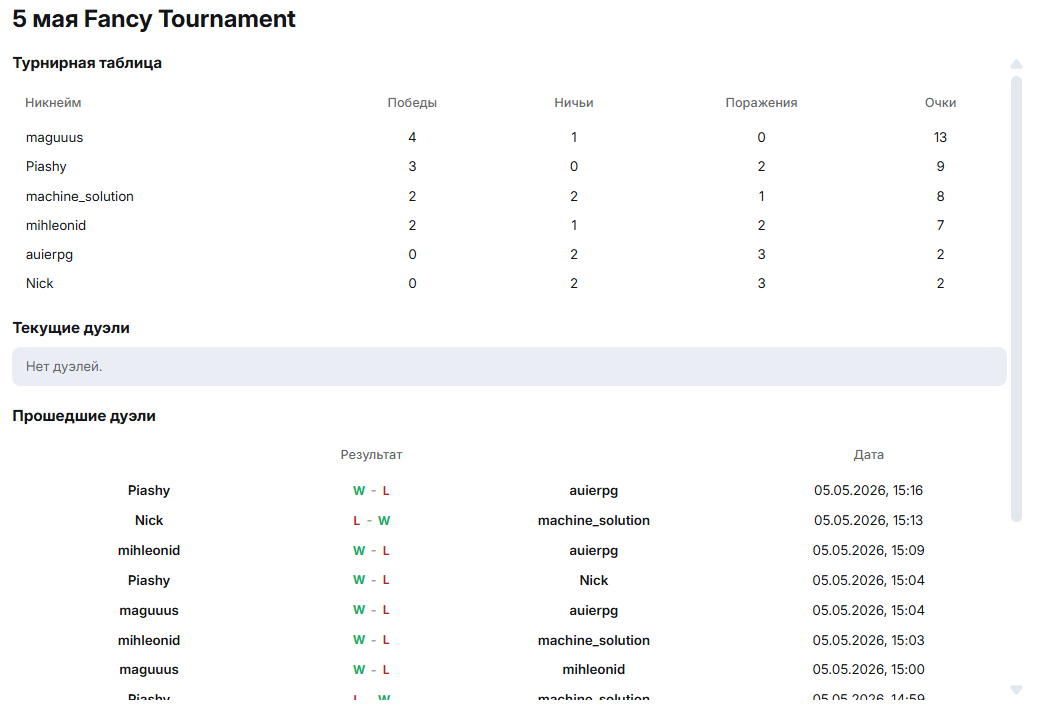
\includegraphics{images/tournament-interface.png}
}
\caption{
\label{tournament-interface}
     Интерфейс турнира.}
\end{center}
\end{figure}

Была спроектирована распределённая микросервисная архитектура системы,
включающая компоненты Frontend, Duely, Taski, Exesh, Analyzer и Dashboard.
Для взаимодействия компонентов использовались HTTP, WebSocket и Kafka.
Разработанная архитектура позволяет масштабировать систему и эффективно распределять вычислительные ресурсы между компонентами.

Автоматическое тестирование решения было рассмотрено в виде ориентированного ацикличного графа Jobs.
Для распределения вычислительных ресурсов был разработан алгоритм планирования Executions,
учитывающий как время существования Execution, так и прогресс его выполнения.
Также был предложен алгоритм распределения Jobs по Workers, позволяющий повысить эффективность использования ресурсов системы.
Проведённое нагрузочное тестирование показало, что система эффективно использует вычислительные ресурсы
и обеспечивает высокую степень параллельности выполнения задач.

Для исполнения пользовательского кода был реализован запуск команд в изолированном окружении с использованием утилиты isolate.
Дополнительно была разработана библиотека filestorage, обеспечивающая хранение и передачу файлов между компонентами системы.

Отдельное внимание в работе было уделено анализу поведения пользователей во время решения задач.
Была поставлена задача оценки степени подозрительности поведения пользователя, сформирован набор поведенческих признаков,
а также реализованы модели машинного обучения.
Полученные результаты показали, что предложенный подход позволяет выявлять отклонения от обычного процесса разработки решения
и может использоваться как вспомогательный инструмент для обнаружения нечестных пользователей, использующих сторонние инструменты.

Разработанная система может быть использована как платформа для проведения дуэлей по спортивному программированию,
а также как основа для дальнейших исследований в области распределённого тестирования решений и анализа поведения пользователей.
В дальнейшем возможным направлением развития является развитие моделей анализа поведения пользователей,
добавление в систему новых и разнообразных типов задач и увеличение набора функциональных требований.
